%\pagestyle{empty}
%\cleardoublepage
%\pagestyle{fancy}
%\pagenumbering{arabic}

\chapter{Trabalhos Relacionados}\label{cap2}

\begin{comment}
Aqui será interessante você fazer uma breve introduÇão e, então, apresentar as distinÇões das respostas abertas: as objetivas (uma duas palavras - sem uma está tudo errado, sem as duas em ordem está tudo errado e etc.), as semi-objetivas (aquelas em que a combinaÇão de palavras causem problemas de possibilidades combinatorial), as redaÇões e o chamados essays. A partir da Figura 2.1, você volta a essa questão do ponto de vista do aprendizado, aqui, nessa introduÇão, penso que pudessa dar uma indicaÇão da dificuldade matemática crescente decorrente das possíveis combinaÇões das palavras.
\end{comment}

Esse capítulo tem como objetivo apresentar os trabalhos publicados que têm abordagems em volta da correção automática e semiautomática de atividades. Dentre os modelos de atividades trabalhados ainda há distinção entre o modelo de escrita livre, como nas redações, e a objetividade das questões curtas alvo desse trabalho. Assim, em torno desse cenário, podemos analisar a influência da forma textual e das técnicas aplicadas em diferentes situações na reprodução do critério de correção.

Várias técnicas foram empregadas para a modelagem de respostas e interpretação dos documentos dos estudantes. O desenvolvimento de formas de descoberta de padrões e/ou busca estatística para compreensão das respostas foram foco do estudo na literatura. Através dos trabalhos elencados em cada metodologia, discutimos os problemas encontrados nas pesquisas inclusive com estudos brasileiros desse tipo de ferramenta. 
%inserir texto adicional comentando os principais trabalhos e métodos

\section{Breve Histórico da Predição de Nota}
A avaliação automática é um processo de classificação de documentos muito comum à partir da inclusão da informática no meio educacional. Um trabalho muito relevante considerado o início desse processo foi o estudo realizado por \citeonline{page1966}. Nesse, Page descreve o \textit{Project Essay Grade - PEG}, que consiste no primeiro corretor completo de redações, apresentado com detalhes posteriormente \cite{page1968}. Além desse tipo de questão, o trabalho iniciou o processo de estudo textual para a avaliação automática, observando apenas os padrões de escrita do aluno. Nesse conjunto observado de padrões estavam o tamanho e quantidade de palavras, frases e parágrafos, número de preposições, conectivos e erros gramaticais, frequência dos sinais gráficos, dentre outros, totalizando 30 variáveis. Basicamente, identificando essas características da escrita em geral e a função das palavras utilizadas pelo autor, o PEG apresentou uma correlação múltipla de 71\% das variáveis coletadas para a nota atribuída.

Dessa forma, iniciaram diversas pesquisas para desenvolvimentos dos sistemas inteligentes para apoio ao processo de avaliação. Conforme \citeonline{wresch1993}, após os trabalhos pioneiros, o avanço da interpretação do texto, com as análises linguísticas, e das técnicas de aprendizado de máquina possibilitaram a criação de melhores ferramentas. Posteriormente, com aplicação de tais técnicas, tornou-se ainda mais evidente a predisposição dos algoritmos no apoio ao processo de correção de questões e avaliação de aprendizagem.

Em 1993, Wresch já destacava o grande aumento do desempenho dos computadores para aplicação desse tipo de reconhecimento. Onde, anteriormente, Page gastava horas de processamento com cartões perfurados foi possível a aplicação em computadores pessoais. Atualmente, com a evolução das técnicas e a especialização dos modelos preditivos, podemos processar grupos de textos em larga escala, sejam redações ou questões discursivas e classificá-las em um curto período de tempo. Além disso, a eficiência do aprendizado nos cursos \textit{online} em massa \cite{gamage2016}, os MOOC's - \textit{Massive Open Online Courses}, aumentaram o potencial da coleta de dados educacionais e favoreceram a produção de sistemas inteligentes que suportem ao aprendiz e ao tutor.

\section{Modelos Preditivos}
À partir do momento que foram desenvolvidos os primeiros métodos, a investigação do conteúdo, os problemas da necessidade de interpretação textual e a integração da computação cognitiva inovaram a pesquisa. A Avaliação Assistida pela Computação (ou \textit{Computer Assisted Assesment}) - CAA \cite{conole2005} ganhou outros aspectos e foi integrada com duas grandes áreas de pesquisa em Educação: \textit{Educational Data Mining} - EDM \cite{romero2010} e \textit{Learning Analytics} - LA \cite{siemens2012}. 

Além da preocupação com o processo de correção, a proximidade entre essas pesquisas definiu um eixo de novas abordagens para os dados educacionais. Conforme \citeonline{spalenza2016TISE}, CAA é definido como qualquer processo que objetive apoiar a correção e a verificação de aprendizagem como tarefa dos professores. Enquanto isso, EDM geralmente é associado aos métodos de identificação de padrões nos dados educacionais de forma a utilizá-los em benefício do aprendizado. Por fim, LA é formado por um conjunto de técnicas para descoberta de informações e recomendação de aprendizado, lidando diretamente com o aluno e técnicas de ajuste curricular. Então, apesar de distintas em seu objetivo, vários sistemas permeiam entre as áreas e usualmente trabalham com os mesmos conjuntos de informações, quando não funcionam em conjunto.

Segundo \citeonline{conole2005}, a aplicação das tecnologias educacionais para apoio à avaliação de aprendizagem, como as de CAA, adicionam eficiência e eficácia para o processo de ensino. Porém, para cada modelagem é atribuído um tipo de atividade e uma forma de interpretação diferente sobre os dados. Esses diferentes tipos de atividade são apresentados na Figura \ref{modelos-atividades}.

\begin{figure}[ht]
\centering
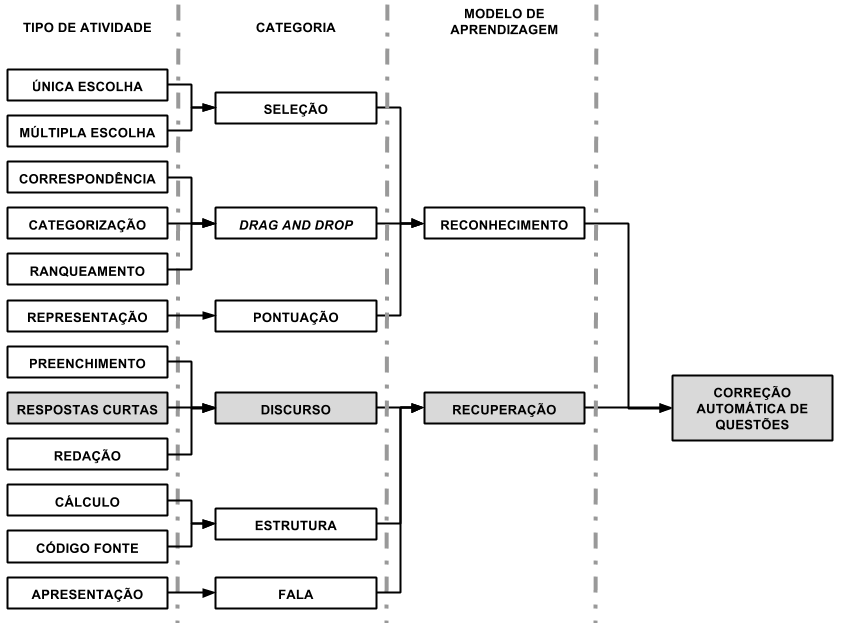
\includegraphics[width=.9\textwidth]{img/atividades.png}
\caption{Tradução da categorização feita por \citeonline{burrows2015} de cada tipo de atividade segundo seu modelo de extração de conhecimento.}
\label{modelos-atividades}
\end{figure}

Dentre as atividades apresentadas na Figura \ref{modelos-atividades}, podemos identificar seis categorias de avaliação e dois modelos de aprendizado. Dentre as categorias, as três que se enquadram na recuperação de informação (discurso, estrutura e fala) exigem maior esforço computacional na busca de informações que permeiam as tarefas dos alunos. Existem subdivisões como as questões de preenchimento, redações e respostas curtas na categoria discurso, pelas diferentes estruturas textuais produzidas pelos alunos. Assim, no nível de automação gerado pelos sistemas, individualmente os tipos de atividade devem passar por análises adequadas para produção de bons resultados.

Estudado por \citeonline{burrows2015}, a profundidade do aprendizado, em tradução literal do ``\textit{depth of learning}'', divide conforme a literatura, cada tipo de atividade em dois grupos: de reconhecimento ou de recuperação. No Brasil, conhecemos por questões abertas e fechadas, como também foi citado pelo autor. Essa divisão então estabelece a diferença entre as atividades que exploram apenas a necessidade de identificação e organização de conteúdo e as que dependem de construção de ideias visando respostas próprias e originais. Definimos, então, a liberdade do aluno na criação do seu conjunto de resposta como a chave para separar atividades que necessitem de maior ou menor conhecimento factual, ou respectivamente, questões abertas ou fechadas.

Ainda na Figura \ref{modelos-atividades}, a categoria recuperação apresenta três tipos de atividades que dependem do discurso do aluno para aquisição das informações. Nessas atividades, especificamente, trabalhamos para encontrar soluções que apoiem o professor na interpretação da escrita dos alunos. Porém, se observarmos as subdivisões respostas curtas, redações e de preenchimento, existem diferenças entre as abordagens e os conhecimentos requisitados. Entretanto, muitos sistemas na literatura não descrevem sua atuação entre os Sistemas Automáticos de Correção de Respostas Curtas - \textit{Automatic Short Answer Grader - ASAG} e os Sistemas Automáticos de Correção de Redações - \textit{Automatic Essay Scorer - AES}. Então, a modelagem computacional é um problema amplo apesar da interpretação de cada modelo na visão do professor. 

Dentro da especialidade dos modelos preditivos, as questões de linguagem natural podem ser distintas pelo tamanho, foco e liberdade do aluno em sua escrita. O tamanho é o principal fator que distingue redações e textos curtos. Esse fator é relevante pois não é claro o limiar entre eles, onde consideramos redações os textos com muitos parágrafos, \citeonline{siddiqi2010} define respostas curtas como ``frases de três ou quatro sentenças'' enquanto \citeonline{sukkarieh2009} como algo ``próximo à 100 palavras''. Para as atividades de preenchimento essa divisão é visível pois delimitam por espaços as poucas palavras que correspondem ao conteúdo. 

Em outra propriedade, o foco, podemos verificar que ao lidar com a produção de texto dos estudantes, as redações são tratadas pelos sistemas nas características de estilo \cite{gutl2007}. Diferentemente das redações, os sistemas ASAG focam no reconhecimento de conteúdo \cite{shermis2013}. Enquanto isso, no modelo de preenchimento, as atividades não baseiam-se no estilo nem no conteúdo em geral, mas sim em palavras específicas. Esse modelo, o de liberdade da questão, é livre de contexto enquanto apenas o essencial precisa ser expresso. Além disso, especificamente no caso das redações, o escritor é livre para a discussão da proposta. Essa liberdade contrasta com os textos curtos, que são inclinados à delimitar o conteúdo abordado no enunciado levando o estudante à uma escrita mais direta e menos opinativa. Essa modelagem textual é resumida por \citeonline{burrows2015} para cada tipo de atividade, com a versão traduzida apresentada na Tabela \ref{tab-propriedades}.

\begin{table}[h]
\centering
\begin{tabular}{l|ccc}
\hline
Tipo de Atividade & Tamanho & Foco & Liberdade Textual \\ 
\hline
Preenchimento & De uma palavra até poucas palavras  & Palavras & Fixo \\
Respostas Curtas   & De uma frase até um parágrafo  & Conteúdo & Fechado \\
Redações  & De dois parágrafos até algumas páginas & Estilo & Aberto \\
\hline
\hline
\end{tabular}
\caption{Propriedades para distinção dos formatos de atividades textuais.}
\label{tab-propriedades}
\vspace{0.5cm}
\end{table}

Assim, dependendo do modelo de atuação são consideradas determinadas características da produção discente para avaliação do conhecimento. Então, para trabalhar especificamente sobre as atividades textuais dos alunos observamos os modelos de avaliação de respostas curtas e redações, apesar de notável a diferença entre estilos.

\begin{comment}
Dentro de uma linha de pesquisa do CAA, o processo de apoio à avaliação, existem métodos distintos que atuam no formato específico da tarefa. Apesar de muitos artigos ainda tratarem os tipos de questão com o mesmo padrão de dados a especificidade de cada abordagem geralmente produz bons resultados. Na análise realizada por \cite{sitthiworachart2008}, por exemplo, vemos uma série de alternativas de correções específicas propostas pela literatura. Nesse encontramos modelos da literatura para tarefas de multipla escolha, diagramas, scripts de programação, grafos e texto. Cada um objetivando apoiar de alguma forma o professor, seja apresentando os erros comuns encontrados nas atividades, realizando avaliação em pares ou criando \textit{feedbacks} automáticos para os estudantes.

Assim, é bem comum trabalhos com domínios específicos pela análise detalhada do problema e a definição de padrões conhecidos de resposta. Podemos citar dentro do problema textual certas diferenças ao lidar com a produção dos estudantes. As redações, por exemplo, podem ser observadas através do estilo da escrita, das conexões entre as palavras, da estrutura sintática, do número de erros ortográficos, da coesão e da proximidade com o tema. Enquanto isso, as questões discursivas, como o objeto aqui trabalhado, geralmente são modeladas pela existência de conteúdos chave para a resposta. Porém, exatamente para identificação de cada um destes subtipos de escrita dos alunos existem as técnicas de busca de informações e interpretação computacional.

\end{comment}

\subsection{Técnicas para Apoio à Avaliação}
Devido a objetividade implícita nas respostas das atividades discursivas curtas, certos métodos foram desenvolvidos para seu processamento. Apesar do carácter avaliativo do texto ser alvo de pesquisas desde a década de 60, o desenvolvimento de ferramentas específicas para cada uma de suas subdivisões ocorreu pouco depois dos anos 2000.

Os bons resultados dos trabalhos focados em modelos particulares de escrita, mudaram a visão sobre os critérios de correção. Os modelos com análise de padrões de escrita, como as respostas únicas e rígidas aguardadas pelos sistemas, foram melhorados para melhor interpretação do texto e análise do conteúdo. Os novos padrões adotados, alteraram a visão mecânica para modos refinados de compreensão computacional da linguagem, muito mais próximos da tarefa humana. \citeonline{mitchell2002} é um dos autores que detalharam a avaliação das respostas curtas. Nesse artigo, o autor apresenta a ferramenta \textit{Automark} na correção de questões de ciência do \textit{Science National Test} através da extração de modelos com análise sintática e semântica. Porém, muitas técnicas foram apresentadas na literatura para identificação dos conjuntos de resposta de cada atividade.

As técnicas aplicadas para localizar relações entre os documentos criados pelos alunos geralmente baseiam-se em duas grandes pesquisas. Uma delas é o Processamento de Linguagem Natural - NLP, que visa definir regras baseadas nas relações estabelecidas na escrita para validá-las junto ao professor ou o material de apoio. Outra grande área trabalhada é o Aprendizado de Máquina - ML. Com essa segunda, a identificação de relações é feita indiretamente pelos algoritmos através de modelos matemáticos e estatísticos. Estabelecendo como são os padrões de avaliação de um conjunto de dados repassados para calibração das informações espera-se que a máquina seja capaz de comparar cada resultado e realizar a avaliação. Geralmente, as técnicas encontradas na literatura misturam a aplicação dessas para reconhecer a relação entre escrita e os padrões. À seguir, descrevemos em alguns grupos de técnicas a influência do ML e do NLP na avaliação de textos curtos até hoje.

\begin{comment}
A seguir
\end{comment}

\subsubsection{Estatística e Base de Dados} \label{ss:STAT}
É muito comum para a avaliação dos dados a requisição de um padrão de resposta esperado para reconhecer regras de escrita e relação entre os objetos citados. Para isso são utilizadas bases de dados como uma forma de extração de conhecimentos sobre o tema proposto. Essas técnicas foram integradas após \citeonline{page1968} empregar estatística pura na pesquisa de avaliação de textos, para realizar uma análise minuciosa das referências encontradas na escrita dos alunos. O objetivo das bases de dados então, é permitir que o \textit{software} tenha conhecimentos em volta do tema trabalhado para ponderar se as afirmações são corretas.

Para estabelecer informações como regras, os sistemas usam relações entre a questão, as respostas e a base de dados. Porém, a base de dados pode ser obtida de diferentes formas: resposta(s) aguarda(s) pelo professor, atividades avaliadas anteriormente por um especialista, bases relacionais (do conteúdo e da linguagem) ou fontes de pesquisa dos alunos. Assim, o uso das bases de dados visam dar maior compreensão em torno do assunto para delinear o tema, comparando modelos segundo a avaliação do professor. Dentre as pesquisas que partem desse pressuposto, \citeonline{datar2004}, faz uso da base relacional Wordnet \footnote{https://wordnet.princeton.edu/} para identificar a relação entre os substantivos encontrados nas respostas. O resultado de sua pesquisa foi o \textit{Essay Grading and Analysis Logic - EGAL}, que faz uso dessa metodologia justamente para encontrar estruturas não articuladas na escrita através do \textit{Gibberish Detector}. Já no processo delineado por \citeonline{gabrilovich2007}, foram localizados 389,202 termos distintos distribuídos em 241,393 artigos do Wikipedia \footnote{https://www.wikipedia.org/} para relacionar os conceitos encontrados na escrita dos estudantes. Outra abordagem com bancos de dados para aquisição de conhecimento foi utilizada por \citeonline{kakkonen2005}, com um banco de redações já avaliadas. Interpretando por pares relacionais previamente avaliados o autor gera análises análogas nos textos.

A proposta de \citeonline{gutl2007} apresenta muitos dos fatores associados às bases de conhecimento para o sistema, chamado de \textit{e-Examiner}. Nesse trabalho ele criou um repositório com questões e respostas com todas as possíveis fontes para elaboração de atividades, correção automática e a criação de comentários avaliativos. De forma parecida, a base de atividades criada e disponibilizada por \citeonline{mohler2011}, foi coletada em turmas de introdução à ciência da computação e estrutura de dados. Para cada atividade discursiva, foi elaborada uma chave de resposta e cada submissão dos alunos foram avaliadas por dois especialistas.

\subsubsection{Processamento de Linguagem Natural - NLP} \label{ss:NLP}
A avaliação das questões discursivas por meio de características da linguagem adentra-se na formação de modelos para aplicação de técnicas de reconhecimento de padrões para avaliar de modo qualitativo e quantitativo a escrita. Ao deparar-se com todas as estruturas que uma linguagem contém, como o português, reconhecidamente complexo, o estudo tende à ser dividido para ser melhor trabalhado. Aos sistemas uma outra linguagem geralmente amplia bastante sua biblioteca ou seu conjunto de dados para compreensão do texto à esse nível. Dessa forma, outras técnicas geralmente não esbarram com esse problema mas não reconhecem diretamente o conteúdo. Conforme \citeonline{manning1999}, para além da análise da sintaxe linguística temos a morfologia que estuda a formação das palavras e a semântica que estuda seu significado. O autor ainda usa a frase de Chomsky ``\textit{colorless green ideas sleep furiously}'' para representar que as figuras de linguagem podem acrescentar complexidade para a compreensão linguística por meio computacional.

Porém, a percepção de que há essa diversidade de informações possíveis através da escrita dos alunos tornou foco o estudo do conteúdo. \citeonline{burstein1998} fez uso de NLP no sistema \textit{e-rater} para compreender a adequação de textos escritos em testes de proficiência em língua estrangeira. Com a aplicação em provas como o GMAT (\textit{Graduate Management Admissions Test}) e o TWE (\textit{Test of Written English}) utilizados pelo autor, geraram bases de dados de referências situacionais e carentes de avaliação. Esse trabalho ainda serviu como referência para o desenvolvimento das pesquisas de \citeonline{wang2008} para o chinês, \citeonline{ishioka2004} para o japonês e o proposto por \citeonline{alfonseca2004} para o espanhol.


O reconhecimento de padrões também esteve muito atrelado a pesquisa de NLP para as redações. A extração de regras e a identificação de conteúdos necessários para o conjunto de respostas permitiu melhorias nos critérios de avaliações conforme existência de trechos chave. Semelhantes as máquinas especialistas, em NLP são criadas estruturas e representações que colaborem com todo o processo de identificação textual. Em geral, trabalhos anteriores com base em NLP extraíam através de regras previamente descritas, como as técnicas estatísticas, o conhecimento inato ao conjunto de dados processado. Hoje, durante a observação textual os sistemas de NLP reconhecem por regras, identificam relações e funções das palavras \cite{pulman2005} ou o próprio conteúdo apresentado pelo aluno em seu conjunto de resposta \cite{cutrone2011}, gerando análises para suporte ao método avaliativo.

O processo delineado por \citeonline{pulman2005}, utiliza um marcador léxico baseado em Processamento de Linguagem Natural - NLP, conhecido por \textit{tagger}, marcando o texto conforme o \textit{PennTreebank dataset} para a formação de padrões buscados com técnicas de aprendizado de máquina. \citeonline{cutrone2011} busca modelos na aplicação das palavras, observando as referências em conjunto. Estudo semelhante também foi realizado por \citeonline{levy2013}, onde para que trechos vinculados sejam encontrados aplica-se inferência léxica e sintática no reconhecimento das construções e palavras que mantém o entendimento das orações.

Um exemplo que mistura Processamento de Linguagem Natural com reconhecimento de padrões em diversos níveis foi produzido por \citeonline{bailey2008}. Nesse trabalho, cada modelo compara as respostas do especialista com a do aprendiz através de um módulo chamado de \textit{CAM - Content Assessment Module}. Através da árvore de dependências produzida por um \textit{chunker} vinculando as diferentes formas de escrita segundo a compatibilidade com a estrutura aguardada. Assim, cada frase escrita da resposta curta é comparada com a do especialista, nos níveis de \textit{tokens}, estrutural e por dependência.

Dessa forma, reconhecimento de padrões quando associado à regras de NLP atua nos sistemas de avaliação de questões discursivas encontrando padrões nas atividades dos estudantes. Porém, existem trabalhos que contornam a aplicação de NLP através do aproveitamento do esforço humano. A proposta de \citeonline{kulkarni2014}, por exemplo, utiliza do conhecimento dos alunos com a avaliação por pares para a criação de \textit{rubrics} \cite{arter2006}, ou seja, para elaborar descrições sobre o modelo de correção da questão. Após identificar características relevantes para avaliação, a própria ferramenta torna-se autossuficiente.

\subsubsection{Análise Semântica Latente - LSA} \label{ss:LSA}
O \textit{Latent Semantic Analysis - LSA}, \cite{deerwester1990} é uma técnica que visa reduzir o conjunto textual através da decomposição vetorial para obter as relações semânticas mais significativas. De forma numérica, portanto, a análise de co-ocorrências textuais retorna referências internas aos grupos de documentos, apresentando de modo sumarizado o contexto presente nas respostas \cite{landauer1998}. A análise semântica entregue, apesar dos fundamentos matemáticos apresenta características próximas ao cognitivismo humano com termos bem relacionados aos documentos processados. Esse modelo foi utilizado por \citeonline{foltz1999} na construção do \textit{Automated Essay Assessor}. Para isso, o LSA foi treinado com o domínio das atividades tornando a semântica foco da avaliação. Com base nesse treinamento os termos selecionados são componentes inter-relacionados com o contexto dos documentos.

Algumas variantes do LSA foram criadas para melhor atender o problema de avaliação. Em sua proposta, \citeonline{kakkonen2005} utilizou o PLSA na melhoria dos problemas encontrados em redações para o método básico. No caso, o autor sugere mudanças no algoritmo tradicional visando contornar a perda de grande parte das informações na seleção de variáveis latentes para muitos documentos. Outros fatores elencados como problemas no método foram limitação do uso de métricas de similaridade e na geração de modelos linguísticos. O \textit{Probabilistic Latent Semantic Analysis} em conjunto com o \textit{Expectation Maximization}, apresentados pelo autor, elaboram modelos linguísticos para uma análise semântica mais profunda do contexto das redações. De forma auxiliar, essa função apresenta resultados conforme dois passos: (I) o de expectativas probabilísticas conforme as variáveis latentes e (II) o de maximização com a atualização das variáveis segundo as probabilidades do primeiro passo. Como meta, esse algoritmo visa construir padrões que melhor caracterizem as redações para uma posterior classificação em técnicas de \textit{Machine Learning}.

O LSA é utilizado na avaliação de textos curtos principalmente pela sua redução de dimensionalidade controlada e a seletividade das características, com \textit{feedback} baseado no contexto \cite{perez2005}. Isso ocorre porque a verificação de conexão semântica entre os poucos pares de palavras definidos com a transformação vetorial apresenta resultados muito bons em respostas diretas. Principalmente quando a relação semântica é observada com apoio de bases de conhecimento como a Wordnet para similaridade entre palavras \cite{mohler2009}. Mais uma modificação ao modelo básico foi estudada por \citeonline{gabrilovich2007} através do \textit{Explicit Semantic Analysis - ESA}. Esse método apoia-se nas técnicas de NLP e uma grande base de conhecimento, o Wikipedia como citado na Seção \ref{ss:STAT}. Assim, cada conteúdo extraído é associado a conceitos da base de dados. O conjunto de textos é então classificado conforme um mapa de conceitos ponderados, com um interpretador semântico e especialmente mais abrangentes para o domínio da base adotada.

\subsubsection{Aprendizado de Máquina - ML}\label{ss:ML}
\textit{Machine Learning} é um conjunto de técnicas que se apoiam na identificação de padrões e extração de informação. Baseiam-se em algoritmos computacionais que produzem modelos de acordo com a distribuição dos dados. Na avaliação de textos curtos, essas técnicas visam compreender a forma de organização textual no espaço \textit{n}-dimensional para reproduzir o comportamento. Então, quanto melhores as informações repassadas pelo especialista humano, há uma tendência de criação de modelos de avaliação mais representativos.

O uso do teorema probabilístico bayesiano foi estudado por \citeonline{rudner2002} para avaliação de redações. De acordo com as características extraídas com os resultados do LSA \cite{landauer1998} e do PEG \cite{page1968}, a análise probabilística da rede bayesiana efetua a avaliação no formato da classificação de documentos clássica. Posteriormente, o trabalho realizado por \citeonline{pulman2005} associou as técnicas de processamento linguístico com o aprendizado de máquina. Foi utilizado \textit{HMM - Hiden Markov Models} treinado como \textit{parser} para reconhecimento das dependências na estrutura da frase. Com a árvore de dependências extraída, os algoritmos \textit{Indutive Logic Programming - ILP}, \textit{Decision Tree Learning - DTL} e \textit{Naive Bayes Classifier - NBC} realizam a avaliação. Porém, para as duas últimas técnicas probabilísticas foram adotadas duas maneiras de análise dos dados. Inicialmente os testes foram realizados sem os dados anotados pelo especialista. Posteriormente, os autores aumentaram o desempenho com indicações da parte essencial da atividade segundo o domínio do especialista tornando a busca bem definida. Porém, esse esforço atribuído ao especialista é maior do que o de correção.

Outras abordagens foram dadas durante a competição da \textit{Hewllet Foundation} no \textit{Kaggle}\footnote{Kaggle Inc. https://www.kaggle.com/}, descrita posteriormente na Seção \ref{ss-databases}. Na época, o competidor \citeonline{conort2012}, utilizou o \textit{ensemble Gxav}, ou seja, os resultados oficiais originam de uma combinação das saídas dos algoritmos de \textit{Machine Learning} na tentativa de obter modelos de classificação mais consistentes do que os individuais. Sua solução foi a quarta colocada da competição. Para alcançar essa posição foram combinados  81 métodos distintos de pré-processamento. Em seu relatório técnico, o autor apresenta a mistura dos métodos \textit{Support Vector Machines - SVM}, \textit{Random Forest - RF} e \textit{Gradient Boosting Machines - GBM} na classificação do \textit{Gxav}. As técnicas, apoiadas em diferentes formas de aprendizado e modelagem, definem por parâmetros de escolha dos resultados a ação tomada para um conjunto geral de atividades. Outro participante da competição, \citeonline{zbontar2012}, também utiliza de um modo de parear os resultados dos algoritmos para obter melhores modelos. Utilizou da técnica de \textit{ensemble} chamada \textit{stacking}, para grupos de termos de 4-\textit{grams} e 6-\textit{grams} com a combinação dos resultados dos modelos de aprendizado estudados. Como modelos de aprendizado, foram utilizados o \textit{Ridge Learner - RL}, \textit{Support Vector Regression - SVR}, \textit{Gradient Boosting Machines - GBM}, \textit{Random Forests - RF} e o \textit{K-Nearest Neighbors}. Com a combinação dos classificadores em subconjuntos de termos, esse autor conseguiu o terceiro lugar da competição.

A metodologia utilizada por \citeonline{roy2016} também é um \textit{ensemble} simples. Apenas dois classificadores: um guiado quantitativamente, relacionando a classificação diretamente à frequência das palavras, e um qualitativamente, com ponderações sobre as melhores e piores características encontradas. Dessa forma, as informações vistas com e sem ponderações enfatizam a importância de características em ambos contextos. A resultante de cada avaliação, portanto, é estimada com a atribuição de pesos entre os dois valores obtidos. Outra maneira de observar a influência das características foi proposta por \citeonline{zehner2016}. O algoritmo proposto estabelece um método de \textit{clustering} para identificação de respostas relacionadas. Uma análise de centroides em \textit{n clusters} pré-definidos pelo professor é utilizada para identificação de grupos de conceitos. Os conceitos extraídos são avaliados pelo professor para validar com ``correto'' ou ``incorreto'' cada centroide de respostas. A classificação final é dada então através da compatibilidade das respostas com os conceitos de cada centroide.

\subsection{Aplicação no Brasil}
No Brasil, poucos estudos tratam especificamente da avaliação de questões discursivas. A metodologia mais abordada, é o LSA, presente em muitos estudos da literatura. Nessa abordagem, a proposta de \citeonline{joaosantos2012} compara a avaliação humana das características com variações da ponderação de termos e da métrica de similaridade. Posteriormente, de forma mais direta, \citeonline{joaosantos2015} compara as divergências entre a avaliação de dois especialistas paralelamente aos resultados obtidos pelo sistema inteligente. Outro autor \citeonline{passero2016}, compara os efeitos do LSA com alguns modelos de análise semântica. Para esse estudo, o modelo com essa técnica teve resultados superiores se comparados com as demais implementações da literatura.

Além do LSA, os estudos nacionais fizeram testes com metodologias alternativas para o problema. \citeonline{oliveira2010} desenvolveu um modelo de \textit{clustering} com grande redução de esforço na avaliação da atividades. Nesse artigo, os padrões encontrados em seis itens avaliados pelo professor foram capazes de reproduzir o modelo de correção para as outras 6000 respostas. 

A  lógica \textit{fuzzy} foi testada por \citeonline{vilela2012} na produção do \textit{SCATeDi}. O ambiente desenvolvido é um sistema especialista que associa um conjunto esperado de termos corretos segundo uma construção de regras do professor. A avaliação ocorre conforme a compatibilidade das respostas com os padrões de conteúdo aguardados. O problema associado aos sistemas especialistas é o esforço maior para organizar regras de correção, enquanto a verificação de completude das respostas, alvo dos demais métodos, geralmente atinge esse objetivo.

O estudo de NLP para análise de respostas discursivas foi alvo da proposta de \citeonline{jariosantos2015}. Porém, como é usual na aplicação dessa técnica, concentraram-se no problema da verificação da sintaxe e da morfologia da construção dos alunos. Esse detalhe é incomum nas atividades curtas pela objetividade da escrita e o caráter restrito  das informações à serem abordadas. Entretanto, o estudo é muito influente para a verificação minuciosa da língua como apresentado na Seção \ref{ss:NLP}. Esse ponto de vista da avaliação contribui muito com a análise do discurso e tem influência significativa na correção de redações. 

Uma ferramenta que trabalha no âmbito da correção de questões discursivas para ensino de SQL foi descrita por \citeonline{figueira2013}. Nesse estudo, o autor realiza a avaliação através de regressores lineares para questões discursivas e códigos SQL. O diferencial dessa análise é a busca pelo comportamento linear das notas atribuídas pelo especialista aos documentos. Nesse método de \textit{Machine Learning}, o coeficiente linear que define cada característica encontrada nos textos dos alunos relaciona-se diretamente à nota recebida.

\subsection{Desafios}
Apesar de ser um estudo encontrado na literatura há décadas, dentro da avaliação automática de questões discursivas existem desafios que permeiam as técnicas utilizadas e a interpretação do conteúdo. Nos primeiros sistemas, a modelagem de questões discursivas era um trabalho realizado com o texto bruto. A partir disso, a busca por equivalência entre resposta e texto dos estudantes falhou por inúmeras vezes na padronização dos documentos e na identificação de sinônimos \cite{leffa2003}. O estudo dessa problemática derivou discussões em torno da identificação do conhecimento na escrita dos estudantes, realizada atualmente em boa parte dos algoritmos. 

A liberdade dada ao aluno, típica das atividades discursivas, permite que todo tipo de texto seja apresentado como resposta, incluindo informações inesperadas. Toda informação que fuja do padrão das respostas é considerado um \textit{outlier}. Esses dados confundem os algoritmos de correção automática e comumente são a grande causa do nível de erro dos sistemas. Existem várias fontes desse tipo de conteúdo como a falta de objetividade das questões, avaliações não criteriosas dos professores, uso de figuras de linguagem e a inclusão de referências externas, encontrados após a categorização por formas distintas de processamento textual. \citeonline{bailey2008}, por exemplo, ao aplicar modelos de linguagem natural a textos curtos, definiu o comportamento do estilo textual segundo a capacidade de compreensão computacional. O estudo gerou a representação da Figura \ref{language-learning}, onde especifica a relação da restrição do discurso das questões de preenchimento e a liberdade das redações.

\begin{figure}[ht]
\centering
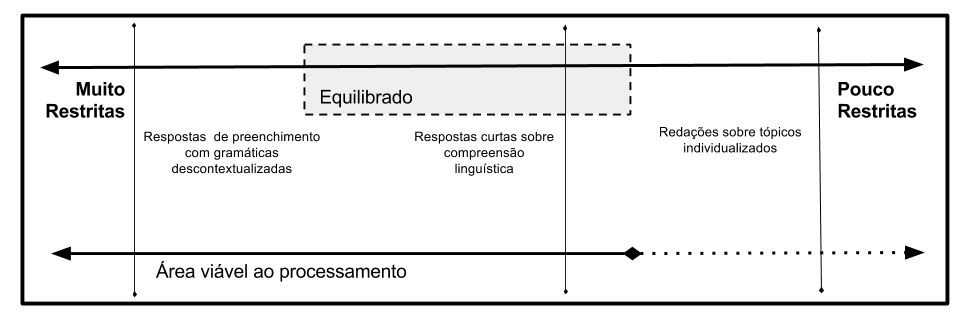
\includegraphics[width=.9\textwidth]{img/aprendizadoNLP.png}
\caption{Tradução da descrição feita por \citeonline{bailey2008} das possibilidades computacionais de processamento das questões discursivas e a limitação dado ao escopo da atividade.}
\label{language-learning}
\end{figure}

Observando o cenário delineado pelo autor, a Figura \ref{language-learning} mostra os problemas nas predições gerados pela a falta de contexto nas respostas e inviabilidade da análise de conteúdo pela liberdade completa de alguns estilos de redação. Assim, o ideal para o processamento de textos é a compreensão do discurso contextualizado com controle do conhecimento ali inserido. Porém, além das nuances da escrita livre como as figuras de linguagem (metáforas, pleonasmos, hipérboles, etc.), o estilo, a padronização, os regionalismos e o sentimento da escrita (negativismo, partidarismo, criticismo, etc.), devemos deixar explicito que definir enunciados que modelem a resposta aguardada faz parte do processo de adequação para a correção automática. Desse modo, definindo questões únicas, focadas e direcionadas ao material estudado é o ideal para esse tipo de análise de dados. Enquanto isso, respostas individualizadas, opinativas e irrestritas ao aluno geralmente não seguem o conteúdo e estrutura e dificultam os processos computacionais. 

Modelos baseados em \textit{Machine Learning}, como o apresentado no Capítulo \ref{cap3} desse trabalho, podem ter problemas como as demais aplicações. A criação de modelos irregulares por \textit{overfitting} ou \textit{underfitting} remetem à padrões que são verossímeis porém representam apenas parcialmente a resposta esperada. Isso implica diretamente na avaliação pelo corte ou adição de informações. É comum aos modelos de definição de padrões a tendência ao erro no processamento de \textit{outliers}, pois não deveriam corresponder à nota ou conteúdo ao qual foi classificada pela avaliação professor. Esse caso ocorre, quando o professor aceita respostas não condizentes com o critério ou quando erroneamente o aluno cria alusões ao conhecimento sem realmente citá-lo.

Apesar de ser uma área de pesquisa já consolidada, a falta de \textit{datasets} abertos ainda é uma limitação para a análise dos algoritmos \cite{burrows2015}. Os dados pessoais presentes no conteúdo e a falta de abordagens tecnológicas para coleta são fatores limitantes. Desse modo, com bases de dados, padrões e métricas distintas cria-se uma barreira para comparação entre sistemas semelhantes.

Na abordagem apresentada neste trabalho, tentamos obter os critérios da classificação do professor. Desse modo, através do processo de seleção de características, contornamos os problemas de representação dos dados e explicamos a distribuição das notas. Gerando uma visualização conseguimos associar termos à notas com modelos avaliativos próximos do especialista e quando a seleção de características não foi efetiva. Assim, podemos avaliar quantitativamente, segundo as métricas de classificação, ao mesmo tempo que é possível interpretar os termos relevantes por nota no papel de usuários do sistema.

O número de \textit{datasets} adquiridos para testes do sistema foram um diferencial. A capacidade do algoritmo de adaptação do pré-processamento para múltiplas linguagens permitiu o uso de bases nacionais e estrangeiras. A falta de bases de dados em português foi contornada com a coleta de dados e suporte aos professores da própria universidade. Enquanto isso, o uso de bases de dados estrangeiras permitiu a comparação do método semiautomático proposto com os resultados de outros sistemas já relatados na literatura.

\section{Visualização dos Resultados}
As técnicas de reconhecimento de padrões, ao serem associadas ao processamento de linguagem natural, frequentemente têm sucesso na representação visual do conhecimento. Alguns trabalhos aplicam dessas técnicas na busca de informações para organizá-las de forma a apoiar o processo de avaliação. No artigo apresentado por \citeonline{gutl2007}, o sistema avaliou cada aluno segundo as respostas sumarizadas, comparando-as com uma base produzida pelo professor do conteúdo através do módulo \textit{ROGUE}. Ao realizar comparações com essa estrutura, é produzido um \textit{feedback} com visualização dos resultados por meio das características relevantes identificadas durante a correção.

Outro sistema de marcações foi proposto juntamente com o \textit{Willow} \cite{perez2006}. Os autores desse estudo definiram uma forma de relacionamento direto entre grupos de resposta do especialista e a produção escrita dos alunos. Com uso das técnicas de NLP, são feitas marcações no texto após a avaliação das respostas curtas pelo LSA, representando a análise semântica em um relatório com as submissões dos alunos.

O trabalho realizado por \citeonline{spalenza2016SBIE} detalha o \textit{mapa de características} como um método de seleção das principais características e encaminhamento de \textit{feedbacks} com as respostas marcadas. Nesse, temos como diferecial a seleção de informações com base apenas na avaliação parcial dada para treinamento dos algoritmos. Dessa forma a representatividade dos termos por nota não é atribuída diretamente pelo professor, mas através do reconhecimento de padrões para trechos de grande relevância. Além de indicar a possível resposta para a questão, as marcações identificam tendências para todas as classes de nota. A representatividade de cada termo nas marcações se dá pela frequência que foi citada pelos alunos por classe.

A visualização dos resultados pode ser caracterizada ainda através de observações não textuais. É o caso do \textit{TreeMap}, utilizado por \citeonline{pissinati2014} para caracterizar o desempenho da avaliação nos grupos de sala de aula. Essa ferramenta gera uma visualização da situação das turmas como apoio para a observação de desempenho dos estudantes. Nesse artigo, o autor ainda elenca e compara seu método com as técnicas clássicas da visualização de dados educacionais. O \textit{TreeMap}, assim como demais modelos, colabora para a tomada de decisões e a autoavaliação do professor.

O \textit{mapa de características}, como sistema aplicado para melhoria e suporte da avaliação de questões discursivas curtas, é apresentado posteriormente no Capítulo \ref{cap4}.